%%%%%%%%%%%%%%%%%%%%%%%%%%%%%%%%%%%%%%%%%%%%%%%%%%%%%%%%%%%
%% Flujo de trabajo

\section{Flujo de trabajo y control de versiones.}\label{flujo:flujo-de-trabajo}

\subsection{Metodología Kanban.}\label{flujo:metodologia-kanban}
\subsubsection{El Tablero Kanban.}\label{flujo:tablero-kanban}
Trello será la herramienta principal para mantener la coordinación del flujo de trabajo a través de un \textbf{Tablero Kanban}. Para el desarrollo del proyecto dividiremos el trabajo en tareas y las iremos incorporando a este tablero dentro de columnas que vienen a representar nuestros procesos de producción.

La idea es anotar cada tarea del proyecto en una tarjeta y agregarla a la columna de la izquierda. Mientras se trabaja en la tarea, su tarjeta va avanzando de izquierda a derecha hasta llegar a la última columna.  

\begin{figure}[h]
	\centering
	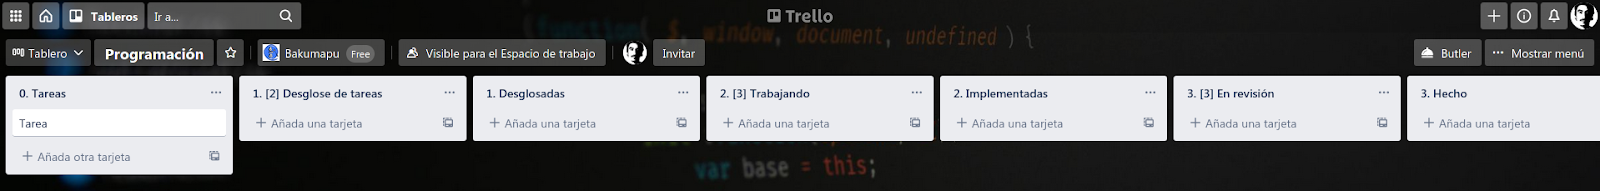
\includegraphics[width=\textwidth]{imágenes/tablero01.png}
	\caption{Tablero Kanban en Trello.}
\end{figure}

\subsubsection{Límites de trabajo y columnas asociadas.}\label{flujo:limites-de-trabajo}
Cada columna tiene asociado un límite máximo de tareas simultáneas (\lsc{WIP}) por lo que si el límite ha sido alcanzado no se podrán incorporar nuevas tareas a la columna hasta haber avanzado una de sus tarjetas a la columna siguiente. Este límite se puede ver en el número dentro de llaves [~].

Al mismo tiempo cada columna tendrá una división vertical, dejando a la izquierda las tareas en proceso y a la derecha las tareas que ya han completado la etapa. El límite es compartido por ambas secciones por lo que independiente de la sección en la que se encuentre la tarjeta, no puede haber más tarjetas que el límite establecido en la columna.

Lamentablemente la plataforma Trello no permite dividir una misma columna en dos secciones, por lo que se añadirá una enumeración al nombre de cada columna que se repetirá en los casos de columnas asociadas. Por ejemplo, sumando las tareas de la columna “2. [5] Trabajando” y las de la columna “2. Terminadas”, solo puede haber 5 tareas simultáneas por lo que no deberemos añadir una sexta.

\begin{figure}[h]
	\centering
	\caption{Límites de trabajo en Trello.}
	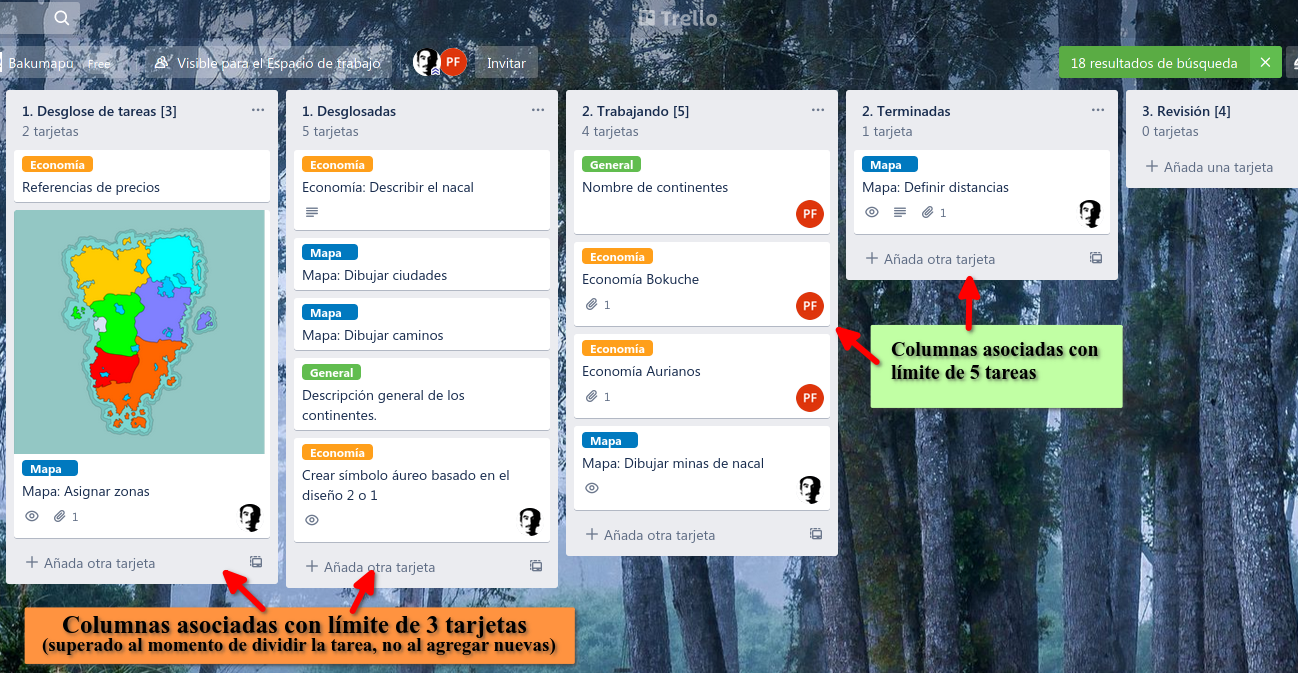
\includegraphics[width=\textwidth]{imágenes/tablero02.png}
\end{figure}

Respetar los límites de cada columna, facilitará la distribución de trabajo en un modelo de entrega continua y nos permitirá tomar decisiones más acertadas y realistas al momento de la planificación.

\subsubsection{Descripción de columnas.}\label{flujo:descripcion-de-columnas}
El funcionamiento de cada columna es bastante sencillo:
\begin{enumerate}
	\item \textbf{Columna Tareas:} Acá dejamos las tareas en sus tarjetas y las ordenamos según prioridad (arriba más urgentes). Solo se debería empezar a trabajar en la tarea superior. La prioridad de las tareas será determinada por el equipo.
	\item \textbf{Columna Desglose de tareas:} Es \textit{muy importante} que las tareas sean descompuestas en tareas sencillas para que no se demoren más de unos días en completarse. Las tareas que entran a esta columna se analizan y dividen en tareas acotadas.
	\item \textbf{Columna Desglosadas:} Aquí las tareas desglosadas esperan hasta que alguien se haga cargo de implementar el código y pasan a la siguiente columna.
	\item \textbf{Columna Trabajando:} Aquí el encargado se anota en la tarjeta y trabaja hasta completarla, pasándola a Terminadas.
	\item \textbf{Columna Implementadas:} Acá quedan las tarjetas con tareas terminadas esperando revisión.
	\item \textbf{Columna En revisión:} Acá van las tareas que se estén revisando. Si tienen problemas o bugs pequeños se resuelven aquí mismo, si tuviera bugs o un problema más grande podría volver a analizarse el desglose con alta prioridad.
	\item \textbf{Columna Hecho:} Aquí van las tareas terminadas. Se eliminan al hacer el merge de un conjunto de features completo a develop (cuando sube la versión).
\end{enumerate}

\subsubsection{Flexibilidad.}\label{flujo:flexibilidad}
Esta es una herramienta que permite tener visualizadas las distintas áreas del proyecto, identificar cuellos de botella y contribuir a la gestión mediante límites de trabajo; no obstante, no debe olvidarse que es solo una guía. Si algo del sistema necesita cambiarse porque va contra el flujo de trabajo, se debe ajustar rápidamente.

\subsubsection{Nombres de Tarjetas.}\label{flujo:nombres-de-tarjetas}
Los nombres de las tareas se deben corresponder con la tarea o funcionalidad a implementar y a su rama asociada en \lsc{GIT}. Más detalles en el apartado \nameref{organizacion:nombres-de-ramas}.

\pagebreak
\subsection{Repositorio.}\label{flujo:repositorio}
El repositorio \lsc{GIT} de Bakumapu se encuentra alojado en la siguiente dirección: \url{https://github.com/polirritmico/Bakumapu}.

La contribución de código será organizada a través del modelo de ramas de función (feature branching) adaptada a un sistema de TDD de entrega continua (más información en el apartado \nameref{principios:principios-de-diseno}).

\subsubsection{Modelo de Ramas de función.}\label{flujo:modelo-de-ramas}
\begin{figure}[H]
	\centering
	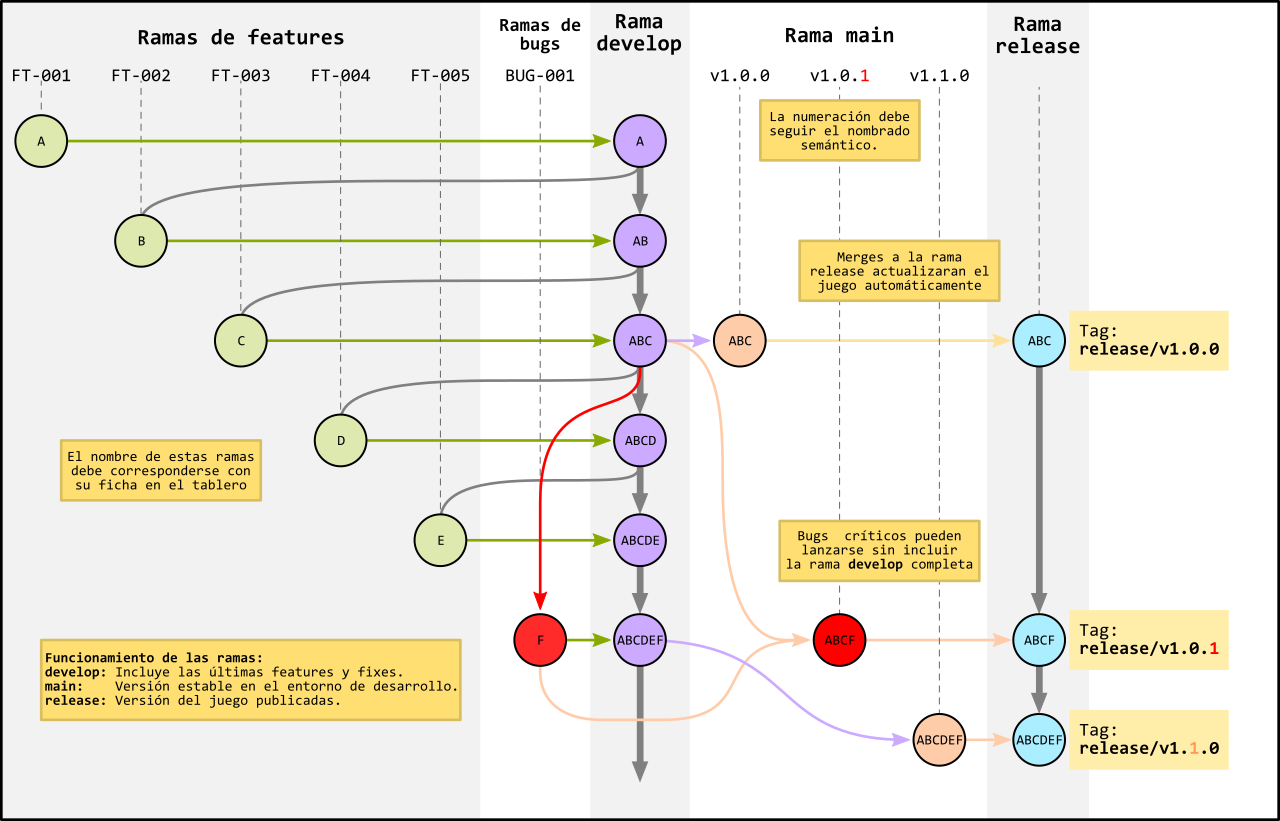
\includegraphics[width=\textwidth]{imágenes/git.png}
	\caption{Ramas en \lsc{GIT}.}
\end{figure}

\noindent\textbf{Ramas principales.}\label{pg:ramas-principales}

Bakumapu contará con 3 ramas principales, \textbf{develop}, \textbf{main} y \textbf{release}.

\begin{enumerate}
	\renewcommand{\labelenumi}{\alph{enumi}.}
	\item \textbf{develop:} Esta rama contará siempre con las últimas funciones implementadas. Es la rama principal del desarrollo ya que para trabajar cada feature, se creará una rama a partir de \textbf{develop}. A medida que se avance esa implementación continuamente se harán merges de vuelta a \textbf{develop} (al menos uno al día)\footnote{Es muy importante este punto porque el tiempo que el código de la rama permanezca fuera de develop puede generar bugs desconocidos al estar aislado de los commit de otras ramas.}. De esta forma se pretende que esté siempre disponible el código completo para no perder la referencia global del proyecto. 
	
	\item \textbf{main:} En esta rama se tratará de mantener el código lo más estable posible. Representa la última entrega del desarrollo y por lo tanto se creará a partir de \textbf{develop} cuando el código haya completado el conjunto de features de cada etapa de implementación del proyecto. Los testers trabajarán en base a esta rama. 
	
	\item \textbf{release:} Se creará a partir \textbf{main} una vez que esta haya sido extensamente probada y depurada. Esta rama será la que pasará el código a producción por eso debe ser la más robusta (por ejemplo deploys automáticos a todas las copias instaladas y conectadas a internet).
\end{enumerate}

\paragraph{Ramas de implementación.}\label{pg:ramas-de-implementacion}
\begin{enumerate}
	\renewcommand{\labelenumi}{\alph{enumi}.}
	\item \textbf{Ramas de features:} Debe crearse una para cada funcionalidad que se quiera implementar a partir del estado actual de la rama \textbf{develop}. El nombre de la rama debe comenzar con “\textbf{ft-}” y corresponderse con el de su tarjeta asociada en el tablero (apartado \nameref{flujo:nombres-de-tarjetas}). La idea es desarrollar test que permitan verificar el funcionamiento de la feature y que deben ser superados antes de dar por concluido el trabajo en la rama. De esta forma se intentará hacer continuos merges hacia \textbf{develop} con la certeza de haber superado los test.
	
	\item \textbf{Ramas de bugs:} Debe crearse una por cada bug encontrado. Dependiendo del bug la rama será creada a partir de \textbf{main}, \textbf{develop} o \textbf{release}. El merge del fix deberá ser hacia \textbf{develop} y si corresponde también a \textbf{release}. El nombre de la rama debe comenzar con “\textbf{bug-}” y corresponderse con el de su tarjeta asociada en el tablero (apartado \nameref{organizacion:nombres-de-ramas}).
\end{enumerate}

Para una información más detallada sobre el funcionamiento de \lsc{GIT} bajo el modelo de ramas de función ver el \href{https://www.atlassian.com/es/git/tutorials/comparing-workflows/feature-branch-workflow}{siguiente enlace} (no olvidar los matices con respecto al trabajo bajo TDD en el apartado \nameref{principios:vision-general-desarrollo}).

\subsubsection{Versionado y nombres semánticos.}\label{flujo:versionado-y-nombres}
Los nombres de las versiones seguirán la nomenclatura de versionado semántico, en este caso \textbf{Bakumapu\_vX.Y.Z} donde cada número representa:
\begin{itemize}[label=-]
	\item \textbf{X:} La versión principal. 0 alfa, 1 release. Si hay cambios no compatibles con la versión anterior, \textbf{X} se incrementa en 1. No debería ser mayor a 1.
	\item \textbf{Y:} La versión menor. Aumenta cuando se agreguen nuevas funcionalidades. Los archivos del usuario (savegames) deben ser siempre compatibles con la versión menor anterior.
	\item \textbf{Z:} La versión de patch. Siempre que se solucione un bug se incrementa y cuando avance la versión menor o principal vuelve a cero.
\end{itemize}

Esta nomenclatura se debe aplicar en las ramas \textbf{main} y \textbf{release}.

\subsubsection{Alternativas al modelo de ramas de función.}\label{flujo:alternativas-al-branching}
Si el flujo bajo el sistema de ramas de función resulta demasiado tedioso o la visualización general del código se pierde con mucha facilidad, ya sea por merges muy complejos o espaciados, se propone como alternativa la metodología de \href{https://es.wikipedia.org/wiki/Entrega_continua}{Entrega continua}.

\subsubsection{Comandos de GIT.}\label{flujo:comandos-de-git}
Este apartado es una referencia rápida a los comandos y configuraciones más comunes en el trabajo con \lsc{GIT}.

\begin{itemize}[label=-]
	\item Configuración:
	\begin{lstlisting}
$ ./config/git/config
	\end{lstlisting}
	
	\begin{lstlisting}
conf[user]
name = USUARIO
email = MAIL_REGISTRADO_EN_GITHUB
[credential]
helper = store
[core]
autocrlf = input
	\end{lstlisting}
	
	\item Credentials en archivo $\sim$/.config/git/credentials (asociado al usuario y al repositorio)
	
	\item Archivos y directorios ignorados por \lsc{GIT} (en .gitignore dentro de Bakumapu):
	\begin{lstlisting}
# Godot-specific ignores
.import/
export/
export.cfg
export_presets.cfg

# Mono-specific ignores
.mono/
data_*/
	\end{lstlisting}
	
	\Needspace{7\baselineskip}
	
	\item Evitar problemas de formato de archivo entre Windows y el resto de sistemas:
	\begin{lstlisting}
$ .gitattributes:
	\end{lstlisting}
	\noindent\begin{minipage}{.45\textwidth}
	\begin{lstlisting}
# Set the default behavior, in
# case people
# don't have core.autocrlf set

* text eol=lf

# Explicitly declare text
# files you want to always
# be normalized and converted 
# to native line endings on
# checkout.

*.godot text
*.tscn text
*.gd text
*.tres text
*.import text
*.md text
*.txt text
*.json text
*.xml text
*.py text
*.c text
*.h text

# binary files that should not
# be modified

# fonts
*.ttf binary
*.otf binary
	\end{lstlisting}
	\end{minipage}\hfill
	\begin{minipage}{.45\textwidth}
	\begin{lstlisting}[escapechar=\%]
# images

*.png binary
*.jpg binary
*.jpeg binary
*.webp binary
*.aseprite binary
*.gif binary
*.xcf binary
*.svg binary
*.kra binary

# sound

*.wav binary
*.ogg binary
*.sf2 binary
*.midi binary
*.amr binary
*.musx binary
*.mp3 binary

# misc

*.zip binary
*.rar binary
*.tar.gz



%
	\end{lstlisting}
	\end{minipage}

	\item Clonar el repositorio en el espacio de trabajo local:
	\begin{lstlisting}
$ git clone https://github.com/polirritmico/Bakumapu
	\end{lstlisting}

	\item - Ver el estado de la rama actual:
	\begin{lstlisting}
$ git status
	\end{lstlisting}
	
	\item Cambiar a una rama (por ejemplo develop):
	\begin{lstlisting}
$ git checkout develop
	\end{lstlisting}
	
	\item Crear una nueva rama en base a la rama actual (ejemplo “ft-01”:
	\begin{lstlisting}
$ git checkout -b ft-01
	\end{lstlisting}
	
	\item Enviar la rama local a Github (origin es un alias de la ruta al repo en github):
	\begin{lstlisting}
$ git push -u origin ft-01
	\end{lstlisting}
	
	\item Agrega todos los cambios al área de pruebas:
	\begin{lstlisting}
$ git add .
	\end{lstlisting}
	
	\item Agrega comentarios al commit:
	\begin{lstlisting}
$ git commit -m descripcion
	\end{lstlisting}
	
	\item Envía los cambios locales de la rama actual a Github:
	\begin{lstlisting}
$ git push
	\end{lstlisting}
	
	\item Actualizar el repositorio local desde Github:
	\begin{lstlisting}
$ git pull
	\end{lstlisting}
\end{itemize}

Referencia rápida para comandos \lsc{GIT} \href{https://rogerdudler.github.io/git-guide}{aquí}.

\subsection{Google Drive.}\label{flujo:google-drive}
Se manejará la \href{https://drive.google.com/open?id=1p8u-1UpXts8OHGRHEZLSIiQrqqx0Y4Kt}{carpeta compartida Bakumapu}, cuyo acceso será proporcionado a todos los miembros del desarrollo. En la raíz de esta carpeta se encuentran los documentos principales del diseño del juego, y las siguientes subcarpetas:
\begin{itemize}
	\item \textbf{Herramientas:} Contiene los instaladores, código fuente, o links de descarga del software discutido en este apartado además de los scripts de desarrollo. También contiene tutoriales para los colaboradores no técnicos del proyecto.
	\item \textbf{Referencias:} Libros, imágenes, documentos, audios, videos y todo material referenciado para el desarrollo, inspiración, discusión o diseño del juego.
	\item \textbf{Historia:} Una especie de repositorio para la narrativa del juego. Contiene documentos sobre la historia, biografía de personajes, arcos narrativos, descripciones, locaciones, historia, trasfondos, etc.
	\begin{itemize}
		\item \textbf{Quest y Diálogos.}
		
		Dentro de la carpeta Historia hay dos subdirectorios relevantes a nivel técnico: Quest y Diálogos. Cada uno contendrá planillas con datos que serán importados a Godot programáticamente, es decir se deberá desarrollar un script o programa que transforme su contenido a \lsc{XML}, \lsc{CSV} o \lsc{JSON} y este sea manejable por Godot con \emph{muy poca} intervención.
		
		Más información de estas herramientas en los apartados \nameref{kit:cutscenes-y-dialogos} y \nameref{kit:quests}. Además estos archivos deberán seguir la convención de nombres detallada en el apartado \nameref{organizacion:nombres-de-archivos}.
	\end{itemize}
\end{itemize}

\subsection{Documentación.}\label{flujo:documentacion}

\subsubsection{El documento de Diseño técnico.}\label{flujo-documento-de-diseno}
Como ya se ha mencionado, la función de este documento es triple:

\begin{enumerate}
	\item Usarse como referencia ante dudas técnicas o de modelado.
	\item Entregar toda la información relevante acerca del flujo de trabajo y del funcionamiento del software para integrar a nuevos miembros del equipo.
	\item Servir de instrumento de diseño.
\end{enumerate}

\paragraph*{¿Qué se documenta?}
En términos generales, el código debe estar debidamente comentado dentro de los archivos correspondientes (revisar apartado \nameref{principios:documentacion-en-codigo}). Para pequeñas modificaciones o adiciones ---sobre todo en relación a funciones y variables---, será suficiente con ajustar estos comentarios en el código. No obstante, para las modificaciones más importantes que involucren cambiar o definir la interacción entre clases o elementos de un ámbito más grande, se deberán mencionar en este documento a modo de referencia técnica en el apartado \nameref{modelado:modelado-del-software}.

\subsubsection{Modificando el documento.}
Como ya se ha mencionado el texto debe modificarse utilizando \LaTeX en cualquier editor de textos. 

Cada modificación a este documento deberá aumentar la numeración de la subversión en 1 (v0.0.1 a v0.0.2). Los primeros 2 índices (v\textbf{0.0.}1) estarán en línea con la última rama \textbf{main} del repositorio. Cada vez que se suba una versión de la rama, se deberá chequear que el documento contenga los cambios relevantes a esa versión, incorporarlos si hace falta y actualizar la versión y volver la subversión a cero (v0.\textbf{5.36} a v0.\textbf{6.0}). El versionado de las ramas se discutirá más adelante en el apartado \nameref{flujo:versionado-y-nombres}.

Dado que la instalación de \LaTeX\ puede ser engorrosa en ciertos contextos, no es necesario compilar una nueva versión con cada cambio de subversión, pero sí será conveniente para los cambios de versiones menores.

Al finalizar las secciones más grandes del código, se debe actualizar el apartado correspondiente.

Es importante aclarar que el objetivo no es una explicación línea a línea de cómo funciona el código, sino una noción general de ámbitos o lógicas más globales. Con señalar el sentido de estas entidades dentro del sistema y su interacción con el resto es suficiente.

\paragraph{Versionado:}
Para cambiar la versión editar el Makefile.

\subsection{LaTeX}
Explicación de comandos básicos de \LaTeX, instalación, compilación. 

\subsection{Documentación dentro del código.}\label{principios:documentacion-en-codigo}
La búsqueda de simplicidad en el diseño también aplica a la documentación del código. Idealmente éste debe estar “autodocumentado”, es decir que los nombres de las variables, métodos y clases den cuenta de manera transparente e intuitiva su rol dentro de la lógica del algoritmo. En los casos más complejos, es de vital importancia añadir comentarios no solo para facilitar la comprensión de líneas más complejas, sino para ayudar al futuro proceso de refactorización y debbuging. \emph{Los nombres largos no lastran la eficiencia del código}.

En cuanto al formato del código dado que \lsc{GDS}cript está basado en Python, además de las propias sugerencias de Godot se recomienda seguir la \href{https://www.python.org/dev/peps/pep-0008/}{guía de estilo PEP-8}.

En especial las siguientes indicaciones:
\begin{itemize}
	\item Límite horizontal de 79 caracteres. 
	\item Separación de 1 línea en blanco entre funciones y 2 entre clases.
	\item Indentación por 4 espacios
	\item Operadores y variables separados por un espacio:\\\small \texttt{var ejemplo = Vector2(2, 5 + PI.get(2))}.
\end{itemize}
